\subsection{Recolección de información}

La información fundamental para este proyecto se obtuvo a través de entrevistas con un profesional experto
en el campo de BI y un coronel de la policía nacional. Además, se elaboró un protocolo técnico para la
recopilación de datos delictivos.
\bigbreak

Es relevante señalar que las respuestas proporcionadas a continuación no son transcripciones literales
de las entrevistas; se han reformulado para ajustarse al contexto de la investigación en curso.

\label{app:entrevista-bi}
\begin{longtable}{|l|p{5cm}|p{5cm}|}
    \caption{Entrevista aplicada al Ing. Rubén Nogales experto en Business Intelligence} \label{tab:entrevista-bi-tab}                                                                                                                                                                                                                                                                                                                                                                                                                                                                                                                                                             \\

    \hline \multicolumn{1}{|c|}{\textbf{N. Pregunta}} & \multicolumn{1}{|c|}{\textbf{Respuesta}}                                                                                                                                                                                                                                                                                                                                                           & \multicolumn{1}{|c|}{\textbf{Observación}}                                                                                                                                                                            \\ \hline
    \endfirsthead

    \multicolumn{3}{c}%
    {{\normalfont \tablename\ \thetable{} -- continuación de la página anterior}}                                                                                                                                                                                                                                                                                                                                                                                                                                                                                                                                                                                                  \\
    \hline \multicolumn{1}{|c|}{\textbf{N. Pregunta}} & \multicolumn{1}{|c|}{\textbf{Respuesta}}                                                                                                                                                                                                                                                                                                                                                           & \multicolumn{1}{|c|}{\textbf{Observación}}                                                                                                                                                                            \\ \hline
    \endhead

    \hline \multicolumn{3}{|r|}{{Continua en la siguiente página}}                                                                                                                                                                                                                                                                                                                                                                                                                                                                                                                                                                                                                 \\ \hline
    \endfoot


    \hline \multicolumn{3}{|p{13cm}|}{{
            \textbf{Conclusión:} La entrevista resalta la importancia crítica de una sólida estructura de datos y un enfoque meticuloso en la
            interpretación y presentación de la información en el ámbito de Business Intelligence (BI). Desde la definición de KPI relevantes hasta la selección
            adecuada de herramientas de análisis y visualización, cada aspecto destaca la necesidad de una estrategia integral que permita convertir los datos en
            acciones concretas. También se señala que una efectiva estrategia de BI requiere no solo tecnología avanzada, sino también una comprensión
            profunda de las necesidades del usuario y una atención constante a la calidad y confiabilidad de los datos.
    }}                                                                                                                                                                                                                                                                                                                                                                                                                                                                                                                                                                                                                                                                             \\ \hline
    \endlastfoot

    1                                                 & Debe ser medible, debe tener la facilidad de ser medido, la variable del KPI debe cumplir con la función de agregación, es decir, en su momento dado pueda generar procesos aritméticos no solo en los hechos sino en las dimensiones.                                                                                                                                                             & La relevancia de un KPI radica en su capacidad de ser medible y agregable, lo que sugiere la importancia de que proporcione una visión general y permita comparaciones.                                               \\\hline
    2                                                 & Semanal es una buena frecuencia a menos que los datos que se generen tengan una gran retroalimentación.                                                                                                                                                                                                                                                                                            & La frecuencia semanal de actualización de informes de BI se sugiere como un equilibrio entre actualización oportuna y necesidad de datos actualizados para la toma de decisiones.                                     \\\hline
    3                                                 & Depende del caso, si los datos necesitan ser comparados, lo mejor son gráficos de barras, si son frecuencias, se deben visualizar histogramas, si en algún momento la información es en función del tiempo, deben ser por medio de gráficos de líneas, y si se desea mostrar porcentajes puede ser mediante un gráfico de pie.                                                                     & La adaptabilidad en el formato de presentación de datos destaca la necesidad de ajustarse al tipo de información para facilitar su comprensión y análisis.                                                            \\\hline
    4                                                 & Que los datos no provean la suficiente información, es decir, el dashboard generado no permita ver claramente lo que se desea para poder tomar decisiones, siendo el principal desafío la organización de los datos.                                                                                                                                                                               & La organización de los datos se identifica como el principal desafío al interpretarlos, lo que destaca la importancia de una estructura clara y comprensible.                                                         \\\hline
    5                                                 & Que sea visual, dinámico, fácilmente entendible, con el cual se pueda realizar filtros y se pueda obtener fácilmente lo que se necesita.                                                                                                                                                                                                                                                           & La efectividad de un sistema de BI para la toma de decisiones se relaciona con su accesibilidad, visualización dinámica y comprensibilidad para los usuarios finales.                                                 \\\hline
    6                                                 & Herramientas para limpieza de datos, completación de datos como cluster, así como herramientas para leer y guardar datos estructurados y no estructurados. También herramientas para visualizar la información como Power BI, Tableau y JS para generar gráficos dinámicos.                                                                                                                        & Se enfatiza la importancia de herramientas de limpieza y visualización de datos, así como la capacidad para manejar datos estructurados y no estructurados.                                                           \\\hline
    7                                                 & Teniendo un buen modelo entidad-relación dimensional, también se debe contar con un modelado de casos de uso dimensional bien establecido.                                                                                                                                                                                                                                                         & Un modelo dimensional sólido y un modelado de casos de uso bien establecido se destacan como clave para abordar problemas de escalabilidad en BI.                                                                     \\\hline
    8                                                 & Se debe realizar un EDA, un Análisis Exploratorio de Datos completo tomando en cuenta que los datos que se obtengan sean de carácter independiente. También definir la distribución de los datos y de cada una de las variables, revisar que los datos sean completos, que no cuenten con ambigüedad, que no haya campos en blanco ni repetidos y también la anonimidadde los datos es importante. & Un análisis exploratorio completo y la garantía de calidad de datos son esenciales para asegurar la confiabilidad de los informes de BI.                                                                              \\\hline
    9                                                 & Definir los KPI obtenidos de los modelados de caso de uso dimensional.                                                                                                                                                                                                                                                                                                                             & La identificación de requisitos de usuarios se sugiere a través de la definición de KPI basados en modelados de casos de uso dimensional, lo que alinea los informes con las necesidades específicas de los usuarios. \\
\end{longtable}
% \begin{longtable}{|l|p{5cm}|p{3cm}|p{3cm}|}
%     \caption{A sample long table.} \label{tab:long}                                                                                                                                                                                                                                                                                                                                                                                                                                                                                                      \\

%     \hline \multicolumn{1}{|c|}{\textbf{First column}} & \multicolumn{1}{c|}{\textbf{Second column}}                                                                                                                                                                                                                                                                                                                                                           & \multicolumn{1}{c|}{\textbf{Third column}} & \multicolumn{1}{c|}{\textbf{Third column}} \\ \hline
%     \endfirsthead

%     \multicolumn{4}{c}%
%     {{\bfseries \tablename\ \thetable{} -- continued from previous page}}                                                                                                                                                                                                                                                                                                                                                                                                                                                                                \\
%     \hline \multicolumn{1}{|c|}{\textbf{First column}} & \multicolumn{1}{c|}{\textbf{Second column}}                                                                                                                                                                                                                                                                                                                                                           & \multicolumn{1}{c|}{\textbf{Third column}} & \multicolumn{1}{c|}{\textbf{Third column}} \\ \hline
%     \endhead

%     \hline \multicolumn{4}{|r|}{{Continued on next page}}                                                                                                                                                                                                                                                                                                                                                                                                                                                                                                \\ \hline
%     \endfoot

%     \hline \hline
%     \endlastfoot

%     1                                                  & Debe ser medible, debe tener la facilidad de ser medido, la variable del KPI debe cumplir con la función de agregación, es decir, en su momento dado pueda generar procesos aritméticos no solo en los hechos sino en las dimensiones.                                                                                                                                                                & 123.456778                                 &                                            \\
%     2                                                  & Semanal es una buena frecuencia a menos que los datos que se generen tengan una gran retroalimentación.                                                                                                                                                                                                                                                                                               & 123.456778                                 &                                            \\
%     3                                                  & Depende del caso, si los datos necesitan ser comparados, lo mejor son gráficos de barras, si son frecuencias, se deben visualizar histogramas, si en algún momento la información es en función del tiempo, deben ser por medio de gráficos de líneas, y si se desea mostrar porcentajes puede ser mediante un gráfico de pie.                                                                        & 123.456778                                 &                                            \\
%     4                                                  & Que los datos no provean la suficiente información, es decir, el dashboard generado no permita ver claramente lo que se desea para poder tomar decisiones, siendo el principal desafío la organización de los datos.                                                                                                                                                                                  & 123.456778                                 &                                            \\
%     One                                                & Que sea visual, dinámico, fácilmente entendible, con el cual se pueda realizar filtros y se pueda obtener fácilmente lo que se necesita.                                                                                                                                                                                                                                                              & 123.456778                                 &                                            \\
%     One                                                & Herramientas para limpieza de datos, completación de datos como cluster, así como herramientas para leer y guardar datos estructurados y no estructurados. También herramientas para visualizar la información como Power BI, Tableau y JS para generar gráficos dinámicos.                                                                                                                           & 123.456778                                 &                                            \\
%     One                                                & Teniendo un buen modelo entidad-relación dimensional, también se debe contar con un modelado de casos de uso dimensional bien establecido.                                                                                                                                                                                                                                                            & 123.456778                                 &                                            \\
%     One                                                & Se debe realizar un EDA, un Análisis Exploratorio de Datos completo tomando en cuenta que los datos que se obtengan sean de carácter independiente. También definir la distribución de los datos y de cada una de las variables, revisar que los datos sean completos, que no cuenten con ambigüedad, que no haya campos en blanco ni repetidos y también la anonimidadde los datos es importante. & 123.456778                                 &                                            \\
%     One                                                & Definir los KPI obtenidos de los modelados de caso de uso dimensional.                                                                                                                                                                                                                                                                                                                                & 123.456778                                 &                                            \\
%     One                                                & abcdef ghjijklmn                                                                                                                                                                                                                                                                                                                                                                                      & 123.456778                                 &                                            \\
%     One                                                & abcdef ghjijklmn                                                                                                                                                                                                                                                                                                                                                                                      & 123.456778                                 &                                            \\
%     One                                                & abcdef ghjijklmn                                                                                                                                                                                                                                                                                                                                                                                      & 123.456778                                 &                                            \\
%     One                                                & abcdef ghjijklmn                                                                                                                                                                                                                                                                                                                                                                                      & 123.456778                                 &                                            \\
% \end{longtable}
\label{app:entrevista-policia}
\begin{longtable}{|l|p{5cm}|p{5cm}|}
    \caption{Entrevista aplicada al teniente coronel de estado mayor Christian Iván Quintana Guerra} \label{tab:entrevista-policia'tab}                                                                                                                                                                                                                                                                                                                                                                                                                                                                                                                                                 \\

    \hline \multicolumn{1}{|c|}{\textbf{N. Pregunta}} & \multicolumn{1}{|c|}{\textbf{Respuesta}}                                                                                                                                                                                                                                                                                                                                                         & \multicolumn{1}{|c|}{\textbf{Observación}}                                                                                                                                                                                   \\ \hline
    \endfirsthead

    \multicolumn{3}{c}%
    {{\normalfont \tablename\ \thetable{} -- continuación de la página anterior}}                                                                                                                                                                                                                                                                                                                                                                                                                                                                                                                                                                                                       \\
    \hline \multicolumn{1}{|c|}{\textbf{N. Pregunta}} & \multicolumn{1}{|c|}{\textbf{Respuesta}}                                                                                                                                                                                                                                                                                                                                                         & \multicolumn{1}{|c|}{\textbf{Observación}}                                                                                                                                                                                   \\ \hline
    \endhead

    \hline \multicolumn{3}{|r|}{{Continua en la siguiente página}}                                                                                                                                                                                                                                                                                                                                                                                                                                                                                                                                                                                                                      \\ \hline
    \endfoot


    \hline \multicolumn{3}{|p{13cm}|}{{
            \textbf{Conclusión:} La entrevista con el teniente coronel Christian Iván Quintana Guerra resalta varios desafíos clave en la gestión
            de seguridad pública, particularmente en la recolección y análisis de datos delictivos. A pesar de la alta demanda ciudadana y la
            implementación de una matriz de Excel para la recopilación continua de datos, existen problemas significativos con la calidad y precisión
            de los reportes debido a la confusión de los ciudadanos entre diferentes tipos de delitos. Además, la obtención de datos completos y
            precisos de los demandantes sigue siendo un reto importante. Es evidente la necesidad de sistemas de gestión de datos más avanzados y
    seguros, así como de una capacitación constante y especializada para el personal policial en nuevas tecnologías. }}                                                                                                                                                                                                                                                                                                                                                                                                                                                                                                                                                                 \\ \hline
    \endlastfoot

    1                                                 & Todos los eventos delictivos que sucedan en el territorio provienen de una demanda ciudadana. Con base en la información recibida del demandante, se recopilan datos georreferenciados de los eventos delictivos, así como horas, fechas, los tipos de personas involucradas en el evento y el modus operandi, lo cual permite realizar los análisis respectivos y tomar las acciones adecuadas. & La precisión en la recopilación de datos es vital para la gestión de seguridad pública, especialmente a través de la georreferenciación y la categorización detallada de eventos.                                            \\\hline
    2                                                 & La calidad aproximada se estima en alrededor del 70\%, tomando en cuenta que los ciudadanos en varios casos confunden los diferentes delitos, siendo el caso más común la confusión entre robo y hurto, lo que resulta en reportes inconsistentes.                                                                                                                                               & La calidad de los datos sobre delitos se ve afectada por la inconsistencia en los reportes ciudadanos                                                                                                                        \\\hline
    3                                                 & Uno de los desafíos que se encuentra comúnmente es que los demandantes proporcionen los datos necesarios para realizar un trabajo más efectivo.                                                                                                                                                                                                                                                  & La obtención de datos completos y precisos de los demandantes representa un desafío significativo para la policía en la recopilación y análisis de datos.                                                                    \\\hline
    4                                                 & Los datos son recopilados de forma continua en una matriz de Excel.                                                                                                                                                                                                                                                                                                                              & Los datos sobre delitos se recopilan en una matriz de Excel de forma continua, sugiriendo una falta de sistemas más avanzados de gestión de datos.                                                                           \\\hline
    5                                                 & El sistema debería proporcionar una información completa sobre un evento delictivo específico con la cual se pueda identificar datos de los agresores, tales como modus operandi, nacionalidad, etnia, altura y contextura. Esto permitiría identificar posibles sospechosos de estar involucrados en algún delito.                                                                              & Existe una necesidad de sistemas de análisis de delitos que proporcionen información detallada sobre los agresores para facilitar la identificación de sospechosos.                                                          \\\hline
    6                                                 & Contar con las protecciones necesarias en las bases de datos.                                                                                                                                                                                                                                                                                                                                    & Se reconoce la importancia de medidas sólidas de seguridad y privacidad de datos, aunque no se especifican detalladamente.                                                                                                   \\\hline
    7                                                 & Esto facilitaría el poder compartir información entre las diferentes unidades con la finalidad de realizar un trabajo más eficiente.                                                                                                                                                                                                                                                             & Los sistemas de análisis de delitos pueden mejorar la colaboración entre unidades policiales al facilitar el intercambio eficiente de información.                                                                           \\\hline
    8                                                 & El nivel de capacitación debe ser alto y constante, dado que uno de los mayores problemas que se enfrenta actualmente es que las promociones más recientes de los miembros de la policía cuentan con conocimientos limitados en cuanto a las nuevas tecnologías.                                                                                                                                 & Se destaca la necesidad de una capacitación constante para el personal policial en el uso efectivo de sistemas de análisis de delitos, especialmente para abordar la brecha tecnológica entre las promociones más recientes. \\
\end{longtable}


La recopilación de información para este proyecto se realizó mediante un protocolo técnico que facilitó la
obtención de datos necesarios para el desarrollo de la propuesta. A continuación, se explica el procedimiento
utilizado para recopilar la información.
\bigbreak

Se diseñó un formulario integrado en una aplicación web para recopilar detalles sobre las víctimas de los incidentes
en la ciudad de Ambato. Este formulario permitirá el registro de información relevante, como el tipo de delito,
la fecha y hora del suceso, y también incluirá un mapa para obtener la ubicación exacta del incidente. Además,
se obtendrán datos a través de alertas de peligro que podrán ser enviadas mediante la aplicación móvil de botón
de pánico que se desarrollara en el proyecto. En la Figura \ref{fig:formulario-recoleccion-datos} se muestra el
formulario  diseñado para la recopilación de información.

\begin{figure}[H]
    \centering
    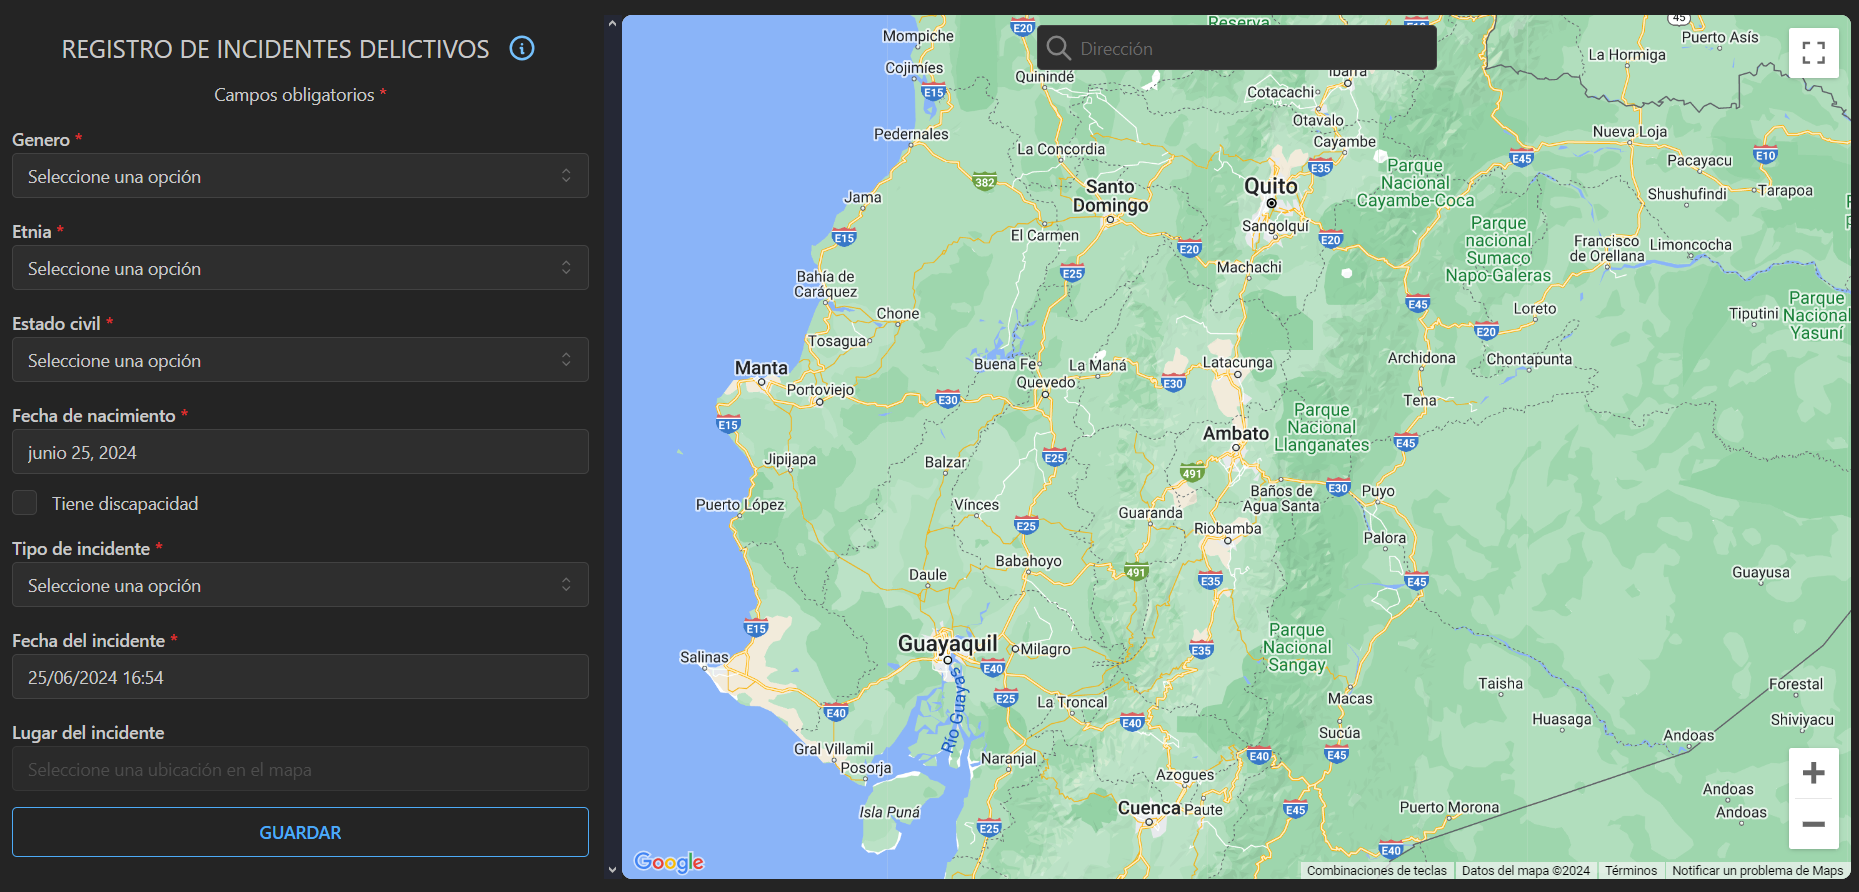
\includegraphics[width=0.8\textwidth]{chapters/II-metodologia/resources/images/formulario-recoleccion-datos.png}
    \caption{Formulario de recolección de datos}
    \label{fig:formulario-recoleccion-datos}
\end{figure}

Mediante este formulario, se recopilarán la cantidad de incidentes establecidos en la muestra, que se estima en 270
incidentes. La información recopilada se utilizará para el análisis de datos y la implementación de la propuesta con
el modelo analítico de BI.